\documentclass[]{article}
\usepackage{lmodern}
\usepackage{amssymb,amsmath}
\usepackage{ifxetex,ifluatex}
\usepackage{fixltx2e} % provides \textsubscript
\ifnum 0\ifxetex 1\fi\ifluatex 1\fi=0 % if pdftex
  \usepackage[T1]{fontenc}
  \usepackage[utf8]{inputenc}
\else % if luatex or xelatex
  \ifxetex
    \usepackage{mathspec}
  \else
    \usepackage{fontspec}
  \fi
  \defaultfontfeatures{Ligatures=TeX,Scale=MatchLowercase}
\fi
% use upquote if available, for straight quotes in verbatim environments
\IfFileExists{upquote.sty}{\usepackage{upquote}}{}
% use microtype if available
\IfFileExists{microtype.sty}{%
\usepackage{microtype}
\UseMicrotypeSet[protrusion]{basicmath} % disable protrusion for tt fonts
}{}
\usepackage[margin=1in]{geometry}
\usepackage{hyperref}
\hypersetup{unicode=true,
            pdftitle={princ\_systems},
            pdfborder={0 0 0},
            breaklinks=true}
\urlstyle{same}  % don't use monospace font for urls
\usepackage{graphicx,grffile}
\makeatletter
\def\maxwidth{\ifdim\Gin@nat@width>\linewidth\linewidth\else\Gin@nat@width\fi}
\def\maxheight{\ifdim\Gin@nat@height>\textheight\textheight\else\Gin@nat@height\fi}
\makeatother
% Scale images if necessary, so that they will not overflow the page
% margins by default, and it is still possible to overwrite the defaults
% using explicit options in \includegraphics[width, height, ...]{}
\setkeys{Gin}{width=\maxwidth,height=\maxheight,keepaspectratio}
\IfFileExists{parskip.sty}{%
\usepackage{parskip}
}{% else
\setlength{\parindent}{0pt}
\setlength{\parskip}{6pt plus 2pt minus 1pt}
}
\setlength{\emergencystretch}{3em}  % prevent overfull lines
\providecommand{\tightlist}{%
  \setlength{\itemsep}{0pt}\setlength{\parskip}{0pt}}
\setcounter{secnumdepth}{0}
% Redefines (sub)paragraphs to behave more like sections
\ifx\paragraph\undefined\else
\let\oldparagraph\paragraph
\renewcommand{\paragraph}[1]{\oldparagraph{#1}\mbox{}}
\fi
\ifx\subparagraph\undefined\else
\let\oldsubparagraph\subparagraph
\renewcommand{\subparagraph}[1]{\oldsubparagraph{#1}\mbox{}}
\fi

%%% Use protect on footnotes to avoid problems with footnotes in titles
\let\rmarkdownfootnote\footnote%
\def\footnote{\protect\rmarkdownfootnote}

%%% Change title format to be more compact
\usepackage{titling}

% Create subtitle command for use in maketitle
\newcommand{\subtitle}[1]{
  \posttitle{
    \begin{center}\large#1\end{center}
    }
}

\setlength{\droptitle}{-2em}

  \title{princ\_systems}
    \pretitle{\vspace{\droptitle}\centering\huge}
  \posttitle{\par}
    \author{}
    \preauthor{}\postauthor{}
    \date{}
    \predate{}\postdate{}
  

\begin{document}
\maketitle

\hypertarget{systems-theory-principles}{%
\section{Systems Theory Principles}\label{systems-theory-principles}}

\hypertarget{stocks-and-flows}{%
\subsection{Stocks and Flows}\label{stocks-and-flows}}

One common approach to explaining how things happen over time is to
identify stocks and flows. Meadows {[}@meadows2009{]} defines both with
the following:

\begin{quote}
A stock is a store, a quantity, an accumulation of material or
information that has built up over time. It may be the water in a
bathtub, a population, the books in a bookstore, the wood in a tree, the
money in a bank, your own self confidence. A stock does not have to be
physical. Your reserve of good will toward others or your supply of hope
that the world can be better are both stocks.
\end{quote}

\begin{quote}
Stocks change over time through the actions of flows. Flows are filling
and draining, births and deaths, purchases and sales, growth and decay,
deposits and withdrawals, successes and failures. A stock, then, is the
present memory of the history of changing flows within the system (18).
\end{quote}

\noindent That last sentence is what makes a stock imply behavior over
time. We speak about stocks by both referring to what they contain right
now but also how they have developed and where they are likely to go.
Also note that stocks do not have to change.

Many organizational phenomena can be viewed as combinations of stocks
and flows. Stocks: Affect {[}@sonnentag{]}, helping behaviors,
depletion, number of customers, justice perceptions, work-family
conflict. Flows: turnover, stressful events, goal assignments. Sometimes
the same thing can be expressed as both a stock and a flow, depending on
how the researcher abstracts the situation. For example, the number of
work tasks could be a stock, where it increases when we are given more
assignments and decreases when we finish them. Or it could be a flow
that leads into something like stress.

The behavior of a stock -- whether it rises, falls, or remains the same
-- depends on the nature of flows. We can learn about stock behavior by
subtracting outflows from inflows. Doing so leads to three general
principles about stocks. They will {[}@cronin2008{]}:

\begin{enumerate}
\def\labelenumi{\arabic{enumi}.}
\tightlist
\item
  rise when inflows exceed outflows
\item
  fall when outflows exceed inflows
\item
  remain the same when inflows equal outflows.
\end{enumerate}

\noindent In other words, stocks change with respect to the summative
properties of their flows. Stocks also set the pace for the dynamics of
the system. Even when flows are changing rapidly, the stock may change
slowly because accumulation occurred over a long period of time.

Figure \ref{stocks} plots a simple stock and flow system over 20 time
periods.

\begin{center}

---------------

Insert Figure \ref{stocks} Here

---------------

\end{center}

\begin{verbatim}
## -- Attaching packages ----------------------------------------------------------------------------------------- tidyverse 1.2.1 --
\end{verbatim}

\begin{verbatim}
## √ ggplot2 3.0.0     √ purrr   0.2.5
## √ tibble  1.4.2     √ dplyr   0.7.6
## √ tidyr   0.8.1     √ stringr 1.3.1
## √ readr   1.1.1     √ forcats 0.3.0
\end{verbatim}

\begin{verbatim}
## -- Conflicts -------------------------------------------------------------------------------------------- tidyverse_conflicts() --
## x dplyr::filter() masks stats::filter()
## x dplyr::lag()    masks stats::lag()
\end{verbatim}

\begin{figure}
\centering
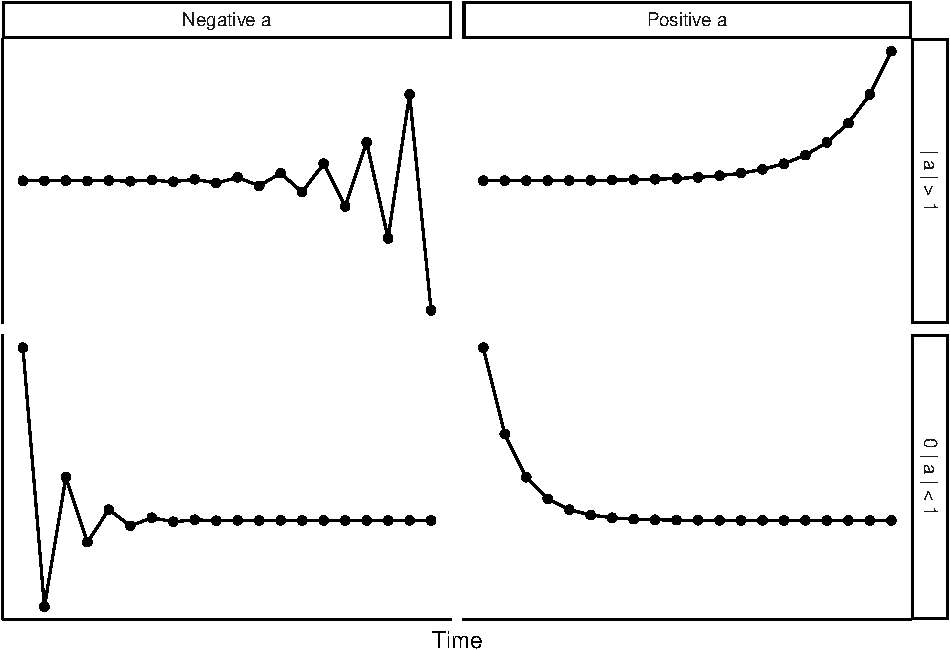
\includegraphics{princ_systems_files/figure-latex/unnamed-chunk-1-1.pdf}
\caption{something\label{stocks}}
\end{figure}

\noindent Beginning at the first time point, inflows are equal to
outflows and the stock therefore sits at zero. Over the first ten time
points, however, outflows remain the same whereas inflows increase. With
inflows exceeding outflows the stock also increases up until time point
ten. At this time, inflows drop back down to five whereas outflows
increase -- leading to a large reduction in the stock. As outflows
continue to rise over time with no counterbalancing movement from the
inflow, the stock ultimately decreases.

Systems theory uses stocks and flows as general labels for each of the
things in the system. Above, we described the behavior of the stocks and
flows with simple terms -- increasing, decreasing, or constant. Systems
theory also provides a more systematic way of describing trajectories
and explaining behavior over time. These are unpacked in an excellent
paper by Monge (1990), and the framework includes trend, magnitude, rate
of change, and periodicity. Each of these is shown respectively in
figure \ref{monge}.

\begin{figure}
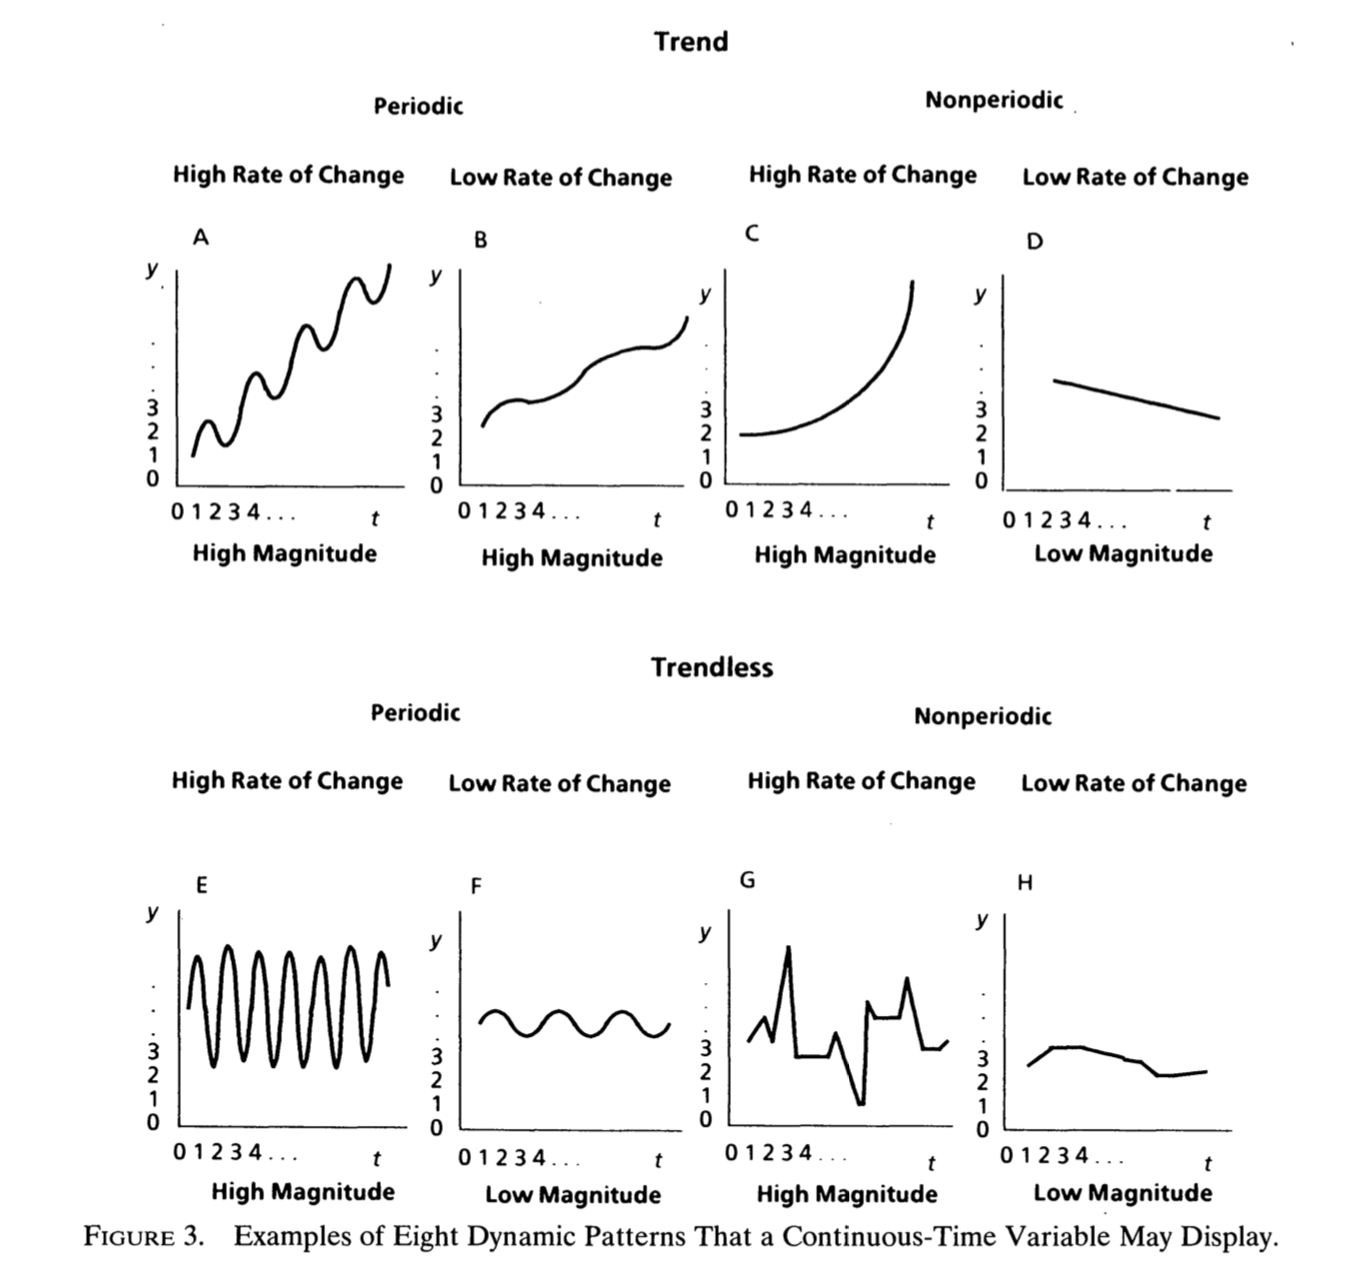
\includegraphics[width=14.25in]{figs/fig_monge1} \caption{something else\label{monge}}\label{fig:unnamed-chunk-2}
\end{figure}

\begin{center}

---------------

Insert Figure \ref{monge} Here

---------------

\end{center}

\hypertarget{trend}{%
\subsection{Trend}\label{trend}}

Dividing figure two into two portions -- the top and bottom -- reveals
differences in trend. All of the panels on the top of figure two have
trend, whereas those on the bottom do not. Trend is the systematic
increase or decrease of a variable over time.

\hypertarget{magnitude}{%
\subsection{Magnitude}\label{magnitude}}

Magnitude is the level, value, or amount of the variable at each time
point -- the number on the \(y\) axis at each respective point in time.
For example, in panel \emph{C} of figure two the magnitude is low at
times 1, 2, and 3, but is high at later points in time. Additionally,
panel \emph{E} and \emph{F} have the same magnitude if we average their
values over time, but panel \emph{E} contains both high and low
magnitude, whereas the magnitude for the trajectory in panel \emph{F}
remains relatively constant.

\hypertarget{rate-of-change}{%
\subsection{Rate of Change}\label{rate-of-change}}

Monge refers to rate of change as ``How fast the magnitude increases or
decreases per one unit of time.'' Panels \emph{G} and \emph{H} reveal
differences in rates of change.

\hypertarget{periodicity-cycles-oscillations}{%
\subsection{Periodicity; Cycles;
Oscillations}\label{periodicity-cycles-oscillations}}

Periodicity is the amount of time before a pattern repeats itself, and
it is equivalent to terms like cycles or oscillations. The most
important piece about periodicity is that it must be couched with
``controlling for trend.'' Notice that panel \emph{A} is periodic
because, after controlling for trend, there are repeated patterns over
time.

\hypertarget{now-two-variables}{%
\subsection{Now two variables}\label{now-two-variables}}

It is of course possible to combine these notions when researchers are
studying processes with more than one variable. For example, a
researcher might describe the magnitude in their presumed dependent
variable with respect to the magnitude of their independent variable, or
the rates of change across the system of variables. When we turn to the
behavior and relationships among a system of variables a few additional
principles are available.

\hypertarget{lags}{%
\subsection{Lags}\label{lags}}

How long does it take for the presumed independent variable to produce
an effect on the outcome? This is the notion of lag.

\hypertarget{permanence}{%
\subsection{Permanence}\label{permanence}}

Once the effect happens, how long does it last?

\hypertarget{feedback-loops}{%
\subsection{Feedback Loops}\label{feedback-loops}}

Systems theory researchers often put feedback loops as a central
component to their discussion or analysis. This idea is also a common
explanation in our own literature. Feedback loops describe processes
where a variable eventually relates back to itself. For example, EXAMPLE
HERE.

Researchers often focus on the behavior that results as a function of
this feedback. When feedback causes the variable to move in the opposite
direction than it initially moved, this is known as negative feedback,
deviation counteraction, or a balancing feedback loop {[}@monge;
@meadows{]}. Here, an initial increase in \(x\) leads to subsequent
changes in the system that, through time, eventually cause \(x\) to
decrease. Now that \(x\) has gone down, more changes happen in the
system that, through time, eventually cause \(x\) to increase.

When feedback, instead, causes the variable to move in the same
direction that it initially moved, this is known as postive feedback,
deviation ampliciation, or a reinforcing feedback loop {[}@monge;
@meadows{]}. Here, changes in \(x\) in one direction lead to eventual
changes in \(x\) in the same direction and thus produce exponential,
explosive, or amplifying behavior.

\hypertarget{summary}{%
\subsection{Summary}\label{summary}}

These systems theory notions are valuable tools to explain and describe
process. Note that we did not cover everything to keep the reading
concise and consistent. For example, @monge also covers discontinuous
systems, so please refer to his excellent paper for an even deeper
discussion. Now we turn to mathematics and statistics and describe
principles from these domains that are used to explain process.


\end{document}
